%! Author = adnansiddiquei
%! Date = 13/12/2023

% Preamble
\documentclass[a4paper,11pt]{article}
\pdfoutput=1

% Packages
\usepackage{jcappub}
\usepackage[T1]{fontenc}
\usepackage{listings}
\usepackage{roboto}
\usepackage{subcaption}

\newcommand{\inlinecode}[1]{\lstinline{#1}}
\lstset{basicstyle=\fontfamily{pcr}\selectfont}


\title{\boldmath M1: Applied Data Science - Coursework Assignment}


% %simple case: 2 authors, same institution
\author{Adnan Siddiquei}
\affiliation{University of Cambridge}

% e-mail addresses: one for each author, in the same order as the authors
\emailAdd{as3438@cam.ac.uk}


\begin{document}
\maketitle
\flushbottom


\section{Section A}\label{sec:section-a}
This section contains the answers to the questions in Section A of the coursework assignment.
Wherever the phrase 'dataset' is used in this section, it refers to \inlinecode{A_NoiseAdded.csv}.
%! Author = adnansiddiquei
%! Date = 13/12/2023

\subsection{Q1 - Dataset A}\label{subsec:dataset-a}
\subsubsection{Question 1a}\label{subsubsec:q1a}
    \begin{figure}[htb]
    \centering
    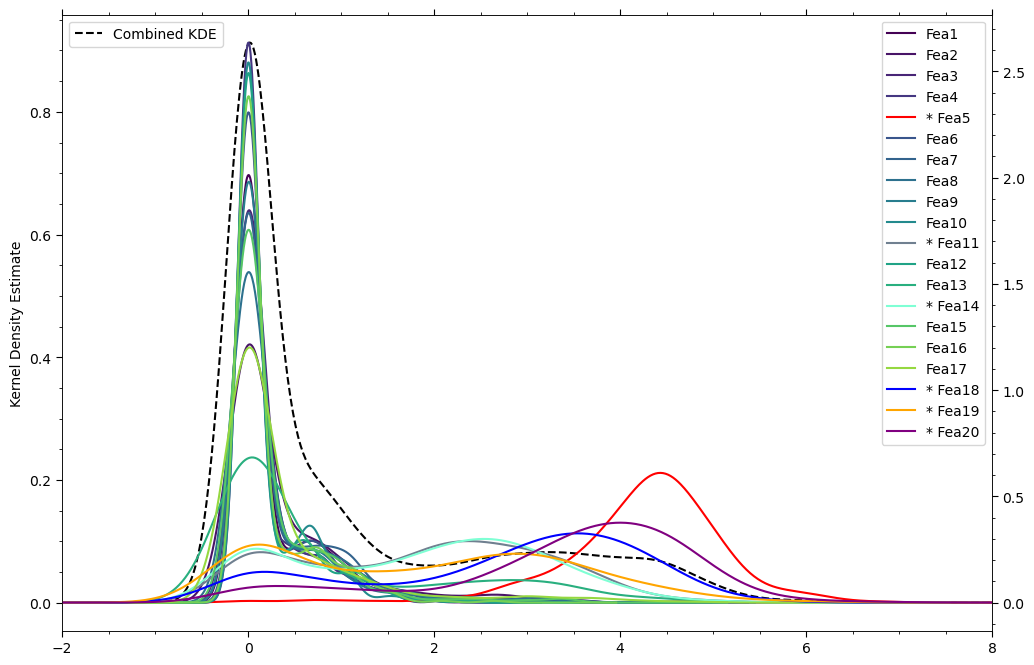
\includegraphics[width=0.9\textwidth]{./figures/q1a}
    \caption{Kernel density estimates of the first 20 features of the \inlinecode{A_NoiseAdded.csv} dataset, with lower
        and higher variance features split into separate plots.}
    \label{fig:q1a}
    \end{figure}

    Fig\eqref{fig:q1a} shows the kernel density estimates of the first 20 features of the dataset.
    The majority of the features are centred around 0 with little variance, except the 6 features on the bottom plot.
    These 6 features are likely to be more discriminative within classification algorithms, as they contain more
    variability.

\subsubsection{Question 1b}\label{subsubsec:q1b}

    \begin{figure}[htb]
    \centering
    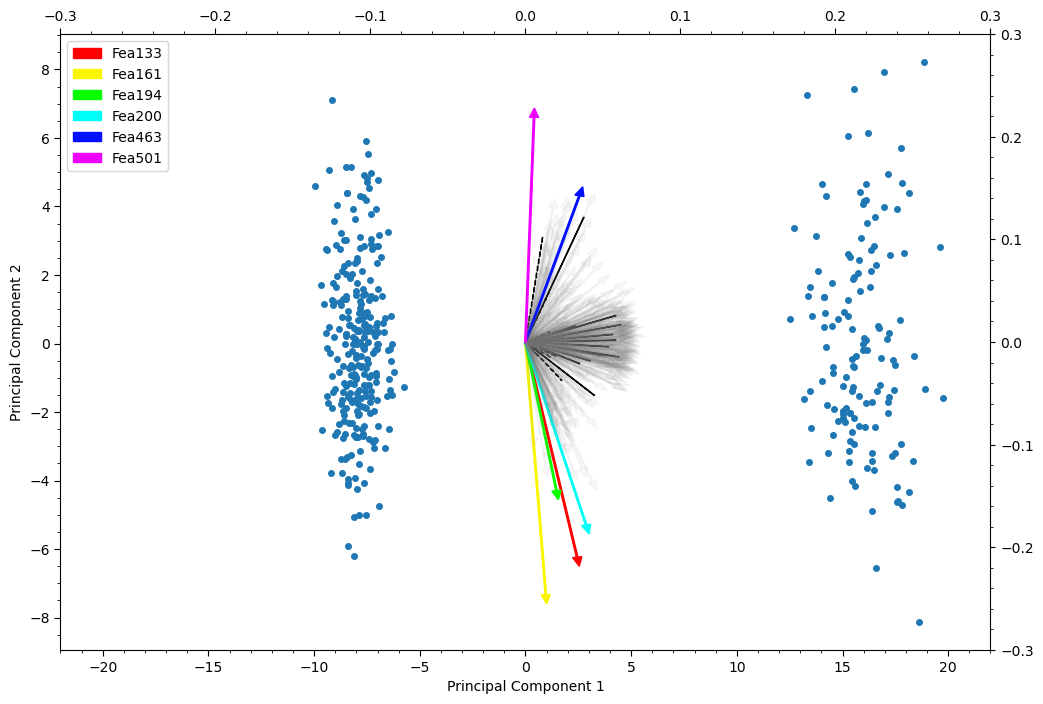
\includegraphics[width=0.9\textwidth]{./figures/q1b}
    \caption{A biplot of the first two principal components in the \inlinecode{A_NoiseAdded.csv} dataset.
        The coloured arrows indicate the first two principal component loading vectors for every feature which contributes to
        either principal component more than 2\%, these are the most discriminative features.
        Every other loading vector has been plotted in very light grey so their general directions and magnitudes are
        visible.
        The loading vectors for the Fig.\eqref{fig:q1a} upper and lower have been plotted in green and red headless
        arrows respectively.
        The loading vectors use the right and top axis of the plot.
        The blue dots indicate the scores for each observation in the dataset for the first two principal components.}
    \label{fig:q1b}
    \end{figure}

    The biplot in Fig\eqref{fig:q1b} shows a PCA of the entire dataset, following standardisation.
    This biplot indicates that the first 20 features are no more discriminative than the rest of the features in the
    dataset, and the assumption that the features in Fig.\eqref{fig:q1a} lower that had more variance would be more
    discriminative is not true as per this plot, as the green loadings tend to stretch further than the red ones.
    Interestingly, whilst the most discriminative features discriminate along PC2, most of the features discriminate
    along PC1, resulting in the large separation along PC1.

\subsubsection{Questions 1c and 1d}\label{subsubsec:q1cd}
    \begin{figure}[htb]
    \centering
    \begin{subfigure}[b]{0.9\linewidth}
        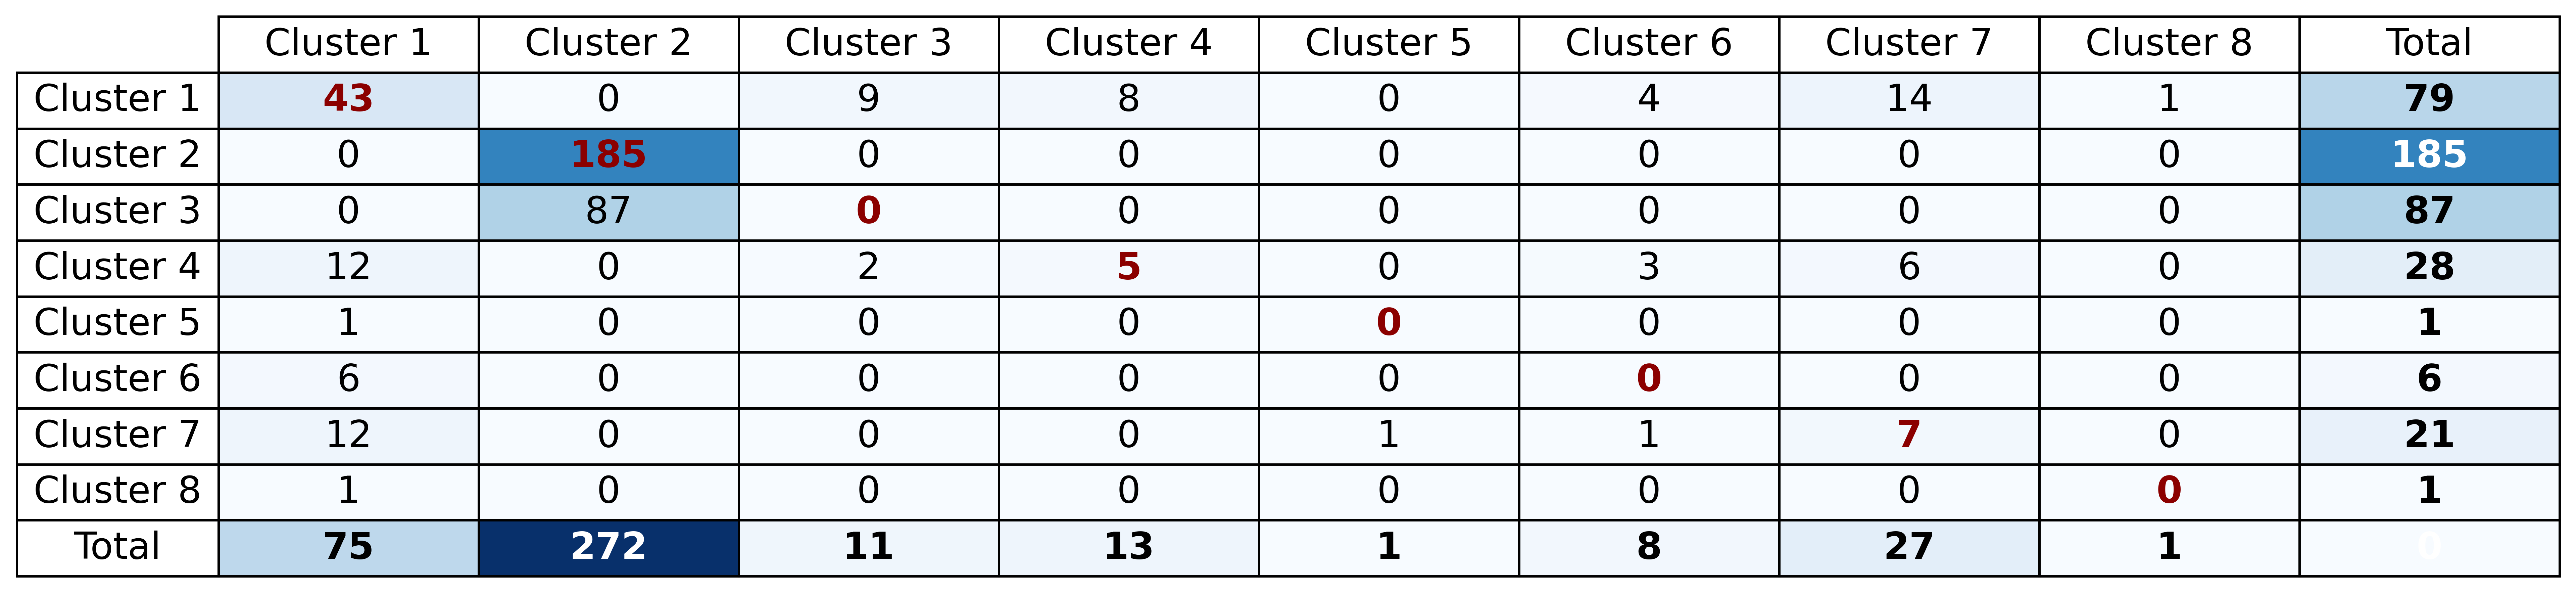
\includegraphics[width=1\textwidth]{./figures/q1c}
        \caption{A contingency table for two k-means clusterings of the \inlinecode{A_NoiseAdded.csv} dataset, with $k=8$,
            the default \inlinecode{scikit-learn} value. 240 of the 408 observations lie on the leading diagonal.}
        \label{fig:q1c}
    \end{subfigure}
    \hfill
    \begin{subfigure}[b]{0.9\linewidth}
        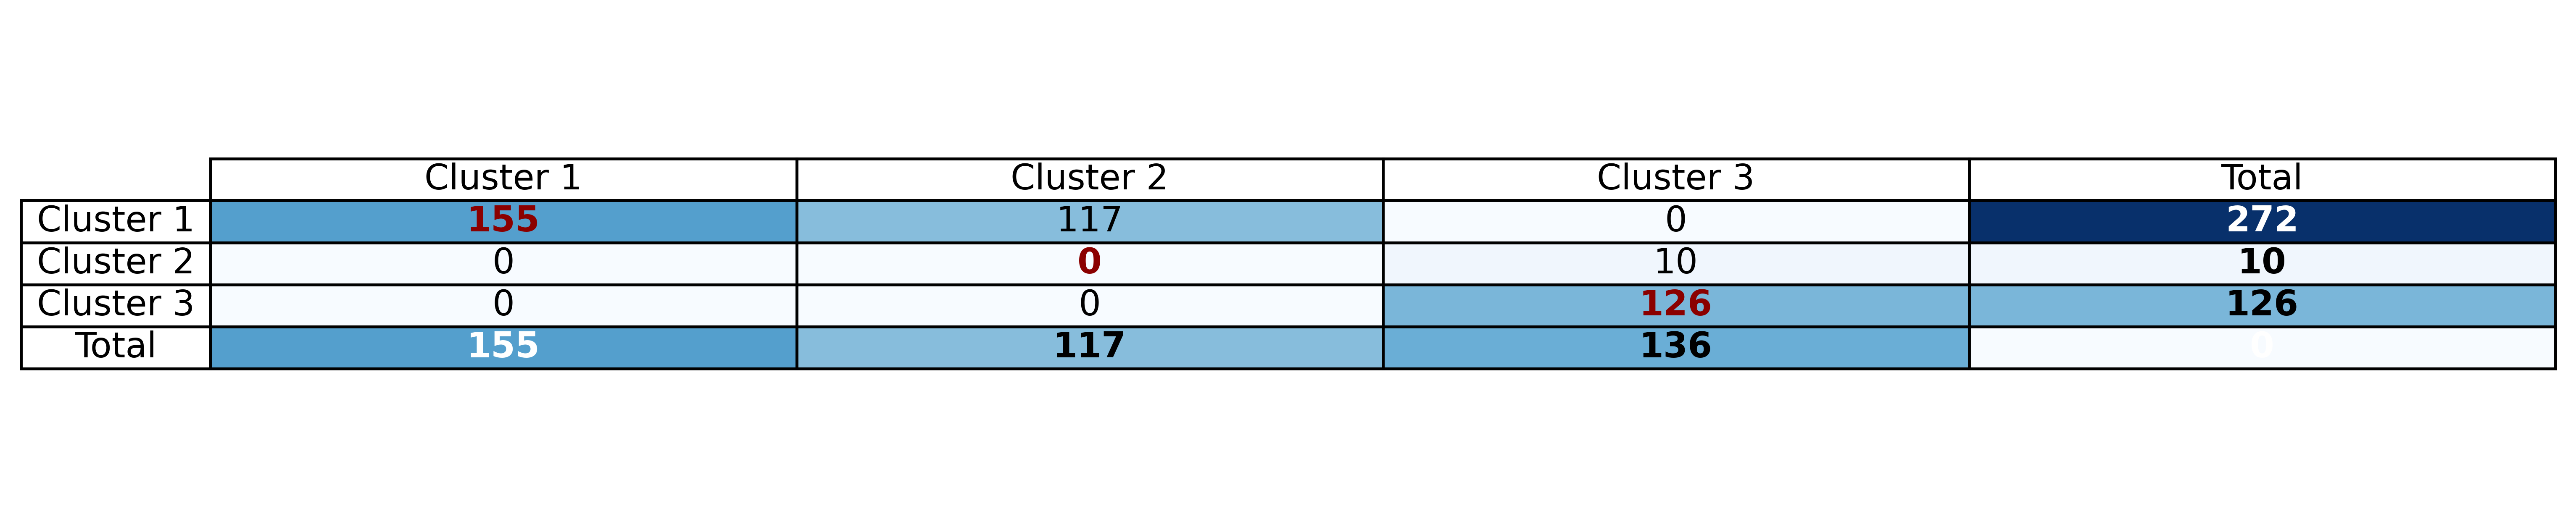
\includegraphics[width=1\textwidth]{./figures/q1d}
        \caption{A contingency table for two k-means clusterings of the \inlinecode{A_NoiseAdded.csv} dataset, with $k=3$.
            281 of the 408 observations lie on the leading diagonal.}
        \label{fig:q1d}
    \end{subfigure}
    \caption{Contingency tables for two k-means clusterings of the \inlinecode{A_NoiseAdded.csv} dataset with number of
        clusters $k=3$ and $k=8$.
        Each feature in the dataset was standardised before clustering.
        \inlinecode{kmeans_1} totals are on the right and \inlinecode{kmeans_2} totals are on the bottom.}
    \label{fig:q1cd}
    \end{figure}

    Fig\eqref{fig:q1c} shows the contingency table for two k-means clusterings of the dataset with $k=8$ and $k=3$.
    Standardisation was applied before clustering as k-means is sensitive to feature scaling.
    The two clusterings (\inlinecode{kmeans_1} and \inlinecode{kmeans_2}) were formed by training two k-means models on
    half of the dataset, and then the other half were mapped onto the learned clusters by assigning new observations
    to the cluster whose centroid is closest to the observation \cite{sklearn-k-means}.
    This is possible because the two models were trained on the same dataset, and so the centroids are in the same
    feature space.
    Labels from each model were re-labelled using the Hungarian algorithm \cite{scipy-linsumopt} \cite{assignment-problem} on
    the pair-wise distances between the centroids of each model, such that label 1 in \inlinecode{kmeans_1} referred to
    label 1 in
    \inlinecode{kmeans_2}.
    This step was crucial, otherwise the contingency table would be meaningless.

    $k=8$ gave a stability of 59\% (the agreement on the leading diagonal), indicating that the two models were
    not very similar, or stable.
    However, \inlinecode{kmeans_1} clustered 85\% of the observations into clusters 1, 2 and 3 and \inlinecode{kmeans_2}
    clustered 86\% of the observations into clusters 1 and 2, indicates that both models correctly identified that most of the data
    lives within a small set of clusters.
    However, the presence of very small clusters indicates that there may be outliers present in the dataset or smaller
    clusters that the large $k=8$ is overfitting to.

    Fig\eqref{fig:q1d} shows the contingency table for two k-means clusterings of the dataset with $k=3$, which gave a
    marginally better stability of 69\%.
    A larger proportion of the observations lie on the leading diagonal compared to $k=8$, which is expected because
    the number of clusters is both smaller and equal to the number of clusters in the classifications column of the
    dataset.
    \inlinecode{kmeans_2} identified 3 distinct clusters whereas \inlinecode{kmeans_1} only identified 2 distinct
    clusters with a few remnant observations in assigned to cluster 2.

\subsubsection{Questions 1e}\label{subsubsec:q1e}
    \begin{figure}[htb]
    \centering
    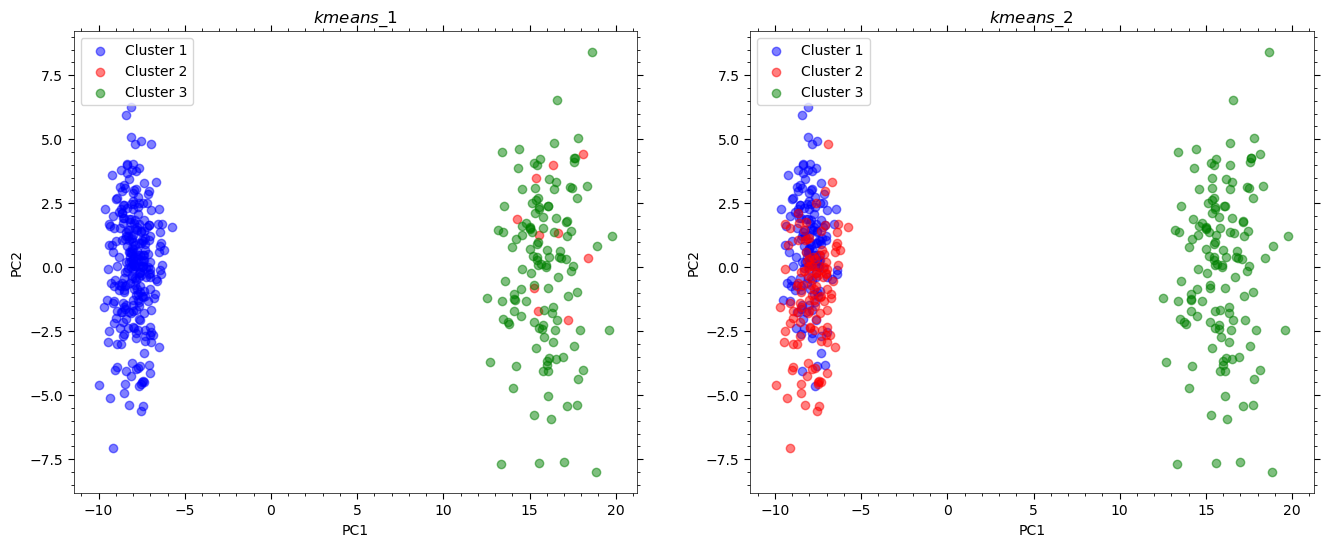
\includegraphics[width=1\textwidth]{./figures/q1e}
    \caption{The k-means clusterings performed with $k=3$, shown on the contingency table in Fig\eqref{fig:q1d}, plotted
        on the first two principal components of the dataset shown in Fig\eqref{fig:q1b}.}
    \label{fig:q1e}
    \end{figure}

    Fig\eqref{fig:q1e} shows the k-means clusterings on the PCA plot shown in Fig\eqref{fig:q1b}.
    Visually, the 2-component PCA indicates that there are two clusters in the dataset.
    Fig\eqref{fig:q1e} also provides subtle evidence in favour of this as well, note the instability of cluster 2 in
    both plots, and it's inability to capture data from both PCA groups at once.
    This, combined with the clear separation of clusters 1 and 3 indicate that there may only be two clusters in the
    dataset, as opposed to the three clusters that the labels indicate.

    Performing k-means before PCA has the advantage of being able to visualise the clusters separation in the original
    feature space.
    However, this might not map well onto the PCA space, as the clusters may be more separable, or separate differently,
    in the original feature space than in the 2-component PCA space.
    It is generally better to perform n-component PCA (or some form of dimensionality reduction or feature selection)
    before k-means as it can reduce noise and mitigate the curse of dimensionality \cite{bellman1957} where distances
    become less meaningful in higher dimensions.

%! Author = adnansiddiquei
%! Date = 13/12/2023

\subsection{Q2 - Dataset B}\label{subsec:dataset-b}
    \begin{figure}
    \centering
    \begin{subfigure}{0.9\textwidth}
      \centering
      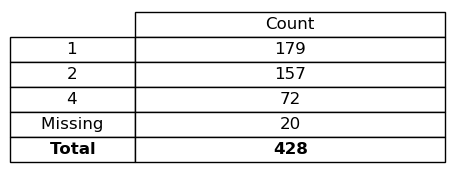
\includegraphics[width=.55\linewidth]{./figures/q2a}
      \caption{Raw \inlinecode{B_NoiseAdded.csv} dataset, before pre-processing. There are 428 observations with 20 missing
        labels and 20 duplicated observations (40 observations involved in the duplication).}
      \label{fig:q2a}
    \end{subfigure}%
    \hfill
    \begin{subfigure}{0.9\textwidth}
      \centering
      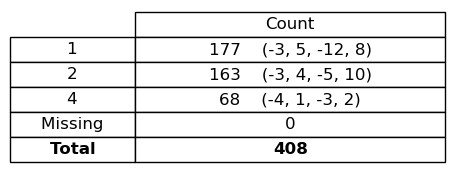
\includegraphics[width=0.55\linewidth]{./figures/q2b_q2d}
      \caption{\inlinecode{B_NoiseAdded.csv} after pre-processing, no missing labels or duplicated observations.
        The 4 numbers in the brackets indicate how the count in each classification changed due to, in order: 1 and 2
        are counts exiting and entering (respectively) the class after correcting for mislabelling; 3 -
        count exiting after dropping duplicates; 4 - count entering after imputation of missing labels.}
      \label{fig:q2bd}
    \end{subfigure}
    \caption{Summary of classifications for the \inlinecode{B_NoiseAdded.csv} dataset before and after pre-processing.}
    \label{fig:q2abd}
    \end{figure}

    Fig.\eqref{fig:q2a} shows the summary of classifications for the \inlinecode{B_NoiseAdded.csv} dataset.
    It was identified that the dataset contained 20 duplicated observations (a total of 40 observations involved in the
    duplication), and 10 of these duplicates contained different labels across the two duplicates. See Appendix
    \ref{appendix:q2} for the full list of duplicates.
    The correct assignment for this mislabelling was determined using multinomal logistic regression on the labelled data
    to predict the labels on the mislabelled data.
    Multinomal logistic regression was then used again to predict the labels for the 20 missing observations, and
    Fig.\eqref{fig:q2bd} shows the new summary of classifications.

    Generally, there are multiple ways to handle missing labels.
    One such way is model based imputation, which was used here.
    This is where an appropriate model is trained on the labelled data to predict the missing labels.
    Another option could be to ignore the data with the missing labels, if the sample size is sufficiently large enough.
    Model based imputation has the advantage of using all the data, however it can introduce bias if the model is not
    a great fit for the data.
    Ignoring the data is advantageous in that it won't create bias if the sample size is large enough.

    Missing at random (MAR) is when the likelihood that a label is missing is independent of the label itself, and
    missing not at random (MNAR) is when the likelihood of the label missing is in some way correlated with the value
    of the label.
    Looking at the 4th number in the brackets of Fig.\eqref{fig:q2bd}, the missing labels in each class as percentages
    of the total count in the respective classes are 4.5\%, 6.1\% and 2.9\% (for 1, 2, and 4 respectively).
    This gives no significant indication of MNAR.

%! Author = adnansiddiquei
%! Date = 13/12/2023

\subsection{Q3 - Dataset C}\label{subsec:dataset-c}
    \begin{figure}
    \centering
    \begin{subfigure}{0.9\textwidth}
        \centering
        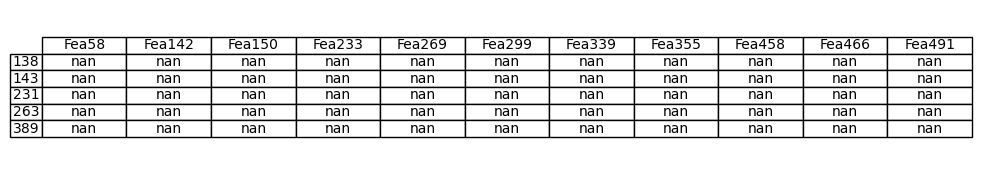
\includegraphics[width=1\textwidth]{./figures/q3a}
        \caption{The samples and features with missing data.}
        \label{fig:q3a}
    \end{subfigure}%
    \hfill
    \begin{subfigure}{0.9\textwidth}
        \centering
        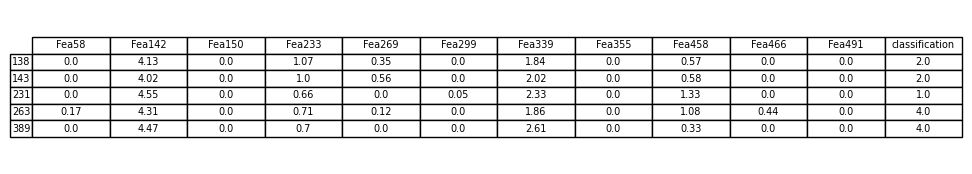
\includegraphics[width=1\textwidth]{./figures/q3c_1}
        \caption{The imputed data.}
        \label{fig:q3c}
    \end{subfigure}
    \caption{Samples and features with missing data, for the \inlinecode{C_MissingData.csv} dataset.}
    \label{fig:q3ac}
    \end{figure}

\subsubsection{Questions 3a and 3b}\label{subsubsec:q3ab}
    Fig\eqref{fig:q3a} shows all the features that have missing values, and all the samples which are missing
    those features.
    There are a few ways to handle missing data.
    A straightforward method is static imputation where every sample missing a given feature, is imputed with the same
    value for that feature, such as the mean of that feature.
    This is computationally inexpensive but can reduce the variance in the dataset and introduce bias if there are many
    missing values.
    Another method is model based imputation where an applicable model is chosen to estimate the value of the missing
    feature for each sample.
    An example is the K Nearest Neighbours approach, where a sample missing a feature is imputed with the mean of the
    K nearest neighbours.
    This can reduce the bias introduced and leave the variance unaffected, but highly dimensional data can often lead
    to less meaningful nearest neighbours, as distance can become less meaningful with more dimensions \cite{bellman1957}.

    Multiple imputation is where the missing data is imputed using a probabilistic model mutliple times, to create
    multiple datasets.
    The multiple imputed values can then either be averaged or the multiple datasets can then be individually analysed,
    Multiple imputation helps capture the uncertainty in what the missing data is, which is useful in the case that
    there is a large amount of missing data.

\subsubsection{Question 3c}\label{subsubsec:q3c}
    \begin{figure}[htb]
    \centering
    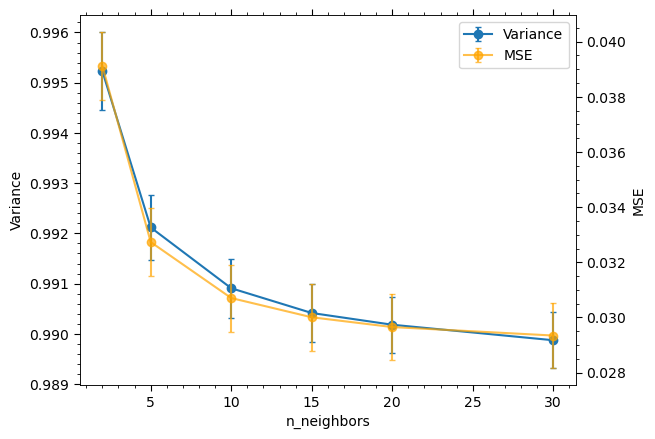
\includegraphics[width=0.9\textwidth]{./figures/q3c_optimise_knn_imputer}
    \caption{Variance and MSE of KNN imputed data, for different values of $k$. The variance is shown as a percentage
        of the original dataset, and the MSE is the mean squared error of predicted values against the true values.}
    \label{fig:q3c_optimise_knn_imputer}
    \end{figure}

    \begin{figure}[htb]
    \centering
    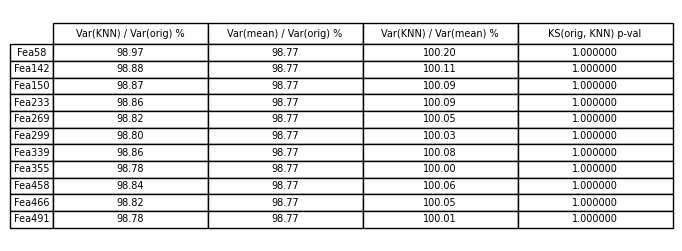
\includegraphics[width=0.9\textwidth]{./figures/q3c_2}
    \caption{A comparison of the variances of each feature after imputation. Column 1 shows the variance of each feature
        after KNN imputation, as a percentage of the original dataset. Column 2 shows this for mean imputation.
        Column 3 compares column 1 against column 2. Column 4 shows the p-value of the Kolmogorov-Smirnov test comparing
        the original dataset to the KNN imputed dataset.}
    \label{fig:q3c_2}
    \end{figure}

    Fig\eqref{fig:q3c_optimise_knn_imputer} was used to optimise the value of $k$ for the KNN imputation, and
    $k=15$ was chosen based on this simulation as further increase in $k$ did not significantly increase accuracy
    (a reduction in MSE).

    Fig\eqref{fig:q3c} shows the imputed data, with aforementioned KNN approach.
    However, PCA was performed first to reduce the dimensionality of the dataset, before the nearest neighbours were
    identified.
    Fig\eqref{fig:q3c_2} shows some summary and comparative statistics of the imputed data, which identifies that
    imputing the missing data did not significantly change the distributions of the features.

\subsubsection{Question 3d and 3e}\label{subsubsec:q3de}
    \begin{figure}[htb]
    \centering
    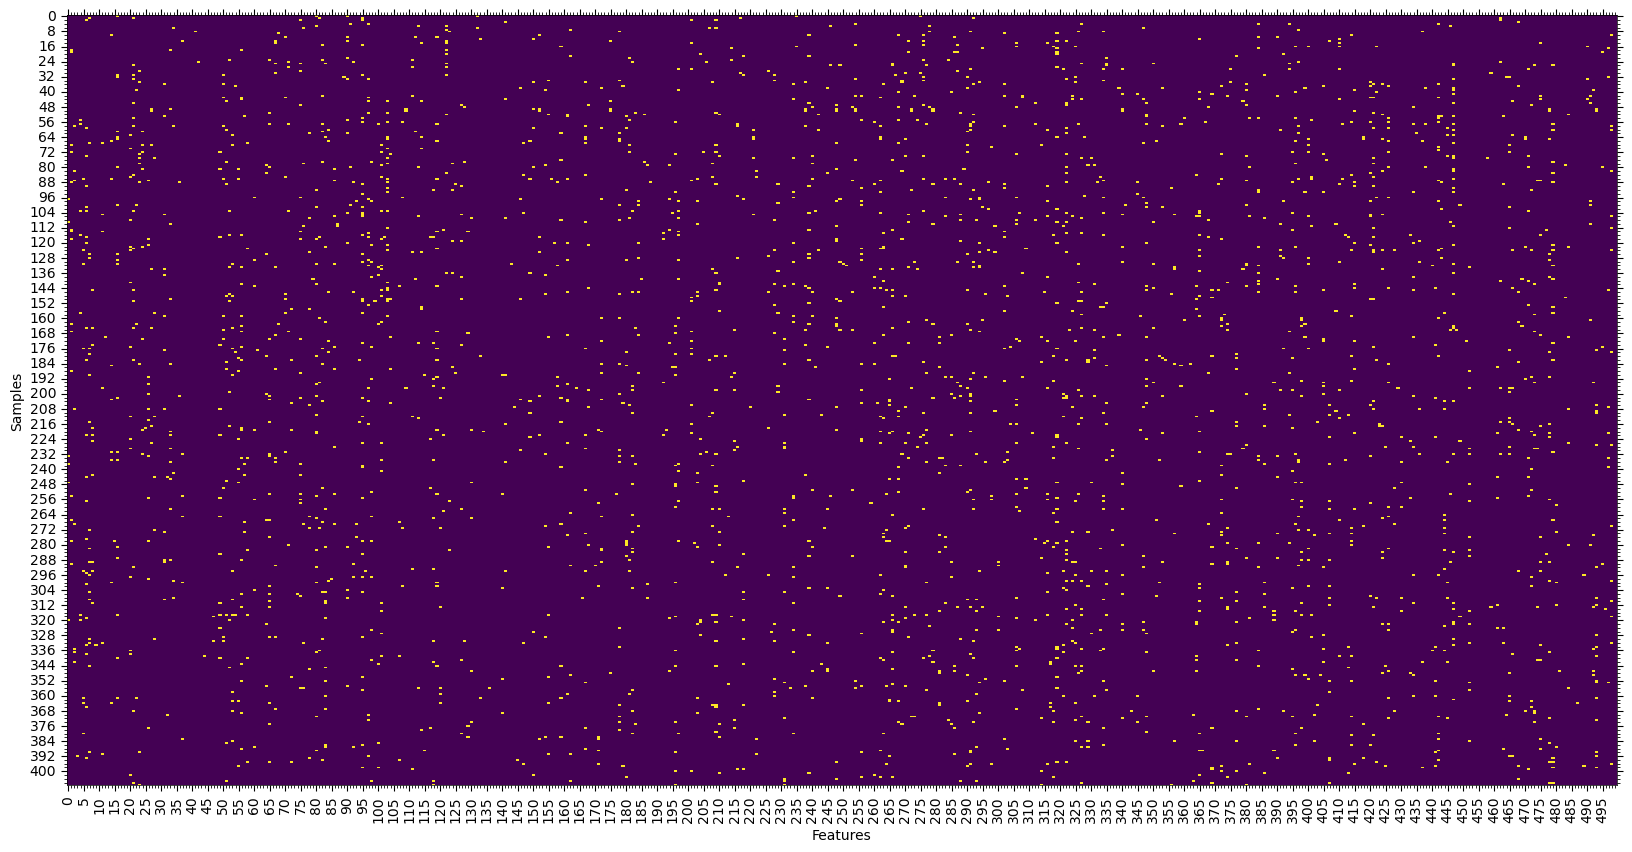
\includegraphics[width=1\textwidth]{./figures/q3d_heatmap}
    \caption{A heatmap of the outliers in the \inlinecode{C_MissingFeatures.csv} dataset. The orange marks indicate an
        outlier value, 2904 outlier values were identified.}
    \label{fig:q3d_heatmap}
    \end{figure}

    \begin{figure}[htb]
    \centering
    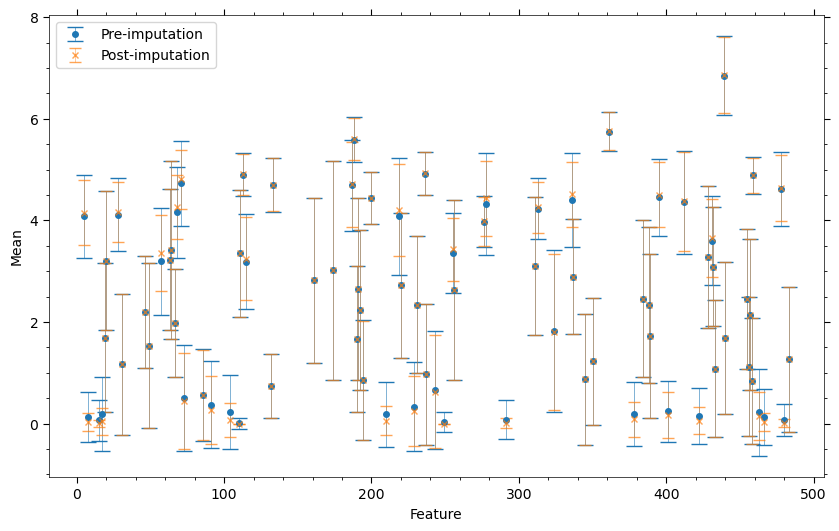
\includegraphics[width=0.9\textwidth]{./figures/q3e}
    \caption{The mean and standard deviation of the 81 most discriminative features in the original
        \inlinecode{C_MissingFeatures.csv} dataset, before and after outlier imputation.}
    \label{fig:q3e}
    \end{figure}

    Outlier values were identified by standardising the data feature-wise, and then identifying any values which were
    more than $3\sigma$ away from the mean.
    Fig\eqref{fig:q3d_heatmap} shows the outliers in the dataset, which shows that the outliers are fairly uniformly
    distributed across the dataset.

    These outliers were treated as missing values and imputed using the same dimensionality reduction and KNN imputation
    approach as utilised in Question 3c for missing values.
    The justification behind this is similar as that for Question 3c, the dataset is clustered and a distance based
    approach is therefore likely to be fruitful, and utilising dimensionality reduction allowed for identification of
    meaningful nearest neighbours.
    Outliers were removed iteratively, with the dataset being re-standardised and outliers being re-computed after each
    iteration.
    The algorithm iterated 8 times, until only 0.27\% of the data lay outside of $3\sigma$, which is the expected
    proportion of data outside of $3\sigma$ for a normal distribution.

    Fig\eqref{fig:q3e} shows the mean and standard deviation of the 81 most discriminative features (identified from
    the PCA loadings) before and after imputing the outliers.
    The variance of the features were reduced after imputation, which was expected, and the reduction in variance in the
    features with means close to zero was more significant as these features were more sparse and therefore more
    likely to have outliers.


\section{Section B}\label{sec:section-b}

\appendix

\section{Q2: Duplicate Observations in \inlinecode{B_NoiseAdded.csv}}\label{appendix:q2}
The duplicated pairs in \inlinecode{B_NoiseAdded.csv}, the number is the sample number:
[[ 74 146], [220 291], [147 409], [ 44 193], [ 66 253], [ 28 260], [384 396], [188 249], [ 83 198], [175 311], [166 424]
 [344 389], [117 297], [351 352], [120 359], [119 382], [100 173], [ 30 101], [ 46 107], [210 305]]


\begin{thebibliography}{99}

\bibitem{sklearn-k-means}
scikit-learn developers,
\textit{\inlinecode{scikit-learn} k-means documentation}.
Available at: \url{https://scikit-learn.org/stable/modules/clustering.html#k-means}
[Accessed: 13-Dec-2023].

\end{thebibliography}



\end{document}
